\documentclass[11pt]{article}
\usepackage{geometry} % Pour passer au format A4
\geometry{hmargin=1cm, vmargin=1cm} % 

% Page et encodage
\usepackage[T1]{fontenc} % Use 8-bit encoding that has 256 glyphs
\usepackage[english,french]{babel} % Français et anglais
\usepackage[utf8]{inputenc} 

\usepackage{lmodern}
\setlength\parindent{0pt}

% Graphiques
\usepackage{graphicx,float,grffile}

% Maths et divers
\usepackage{amsmath,amsfonts,amssymb,amsthm,verbatim}
\usepackage{multicol,enumitem,url,eurosym,gensymb}

% Sections
\usepackage{sectsty} % Allows customizing section commands
\allsectionsfont{\centering \normalfont\scshape}

% Tête et pied de page

\usepackage{fancyhdr} 
\pagestyle{fancyplain} 

\fancyhead{} % No page header
\fancyfoot{}

\renewcommand{\headrulewidth}{0pt} % Remove header underlines
\renewcommand{\footrulewidth}{0pt} % Remove footer underlines

\newcommand{\horrule}[1]{\rule{\linewidth}{#1}} % Create horizontal rule command with 1 argument of height

\begin{document}

\setlength{\columnseprule}{1pt}

\textbf{Nom, Prénom :} \hspace{8cm} \textbf{Classe :} \hspace{3cm} \textbf{Date :}\\
\vspace{-0.8cm}
\begin{center}
  \textit{Les mathématiques ne sont une moindre immensité que la mer.}  - \textbf{Victor Hugo}
\end{center}
\vspace{-0.8cm}

\subsection*{Connaissances}

\begin{enumerate}
  \item[1.] Donner la définition de deux triangles semblables.
  \item[2.] Donner la propriété sur la somme des angles dans un triangle. 
\end{enumerate}



\subsection*{Exercices types}

\begin{multicols}{2}

\subsubsection*{Ex1}

Démontrer que les triangles sont semblables.

\begin{figure}[H]
      \centering
      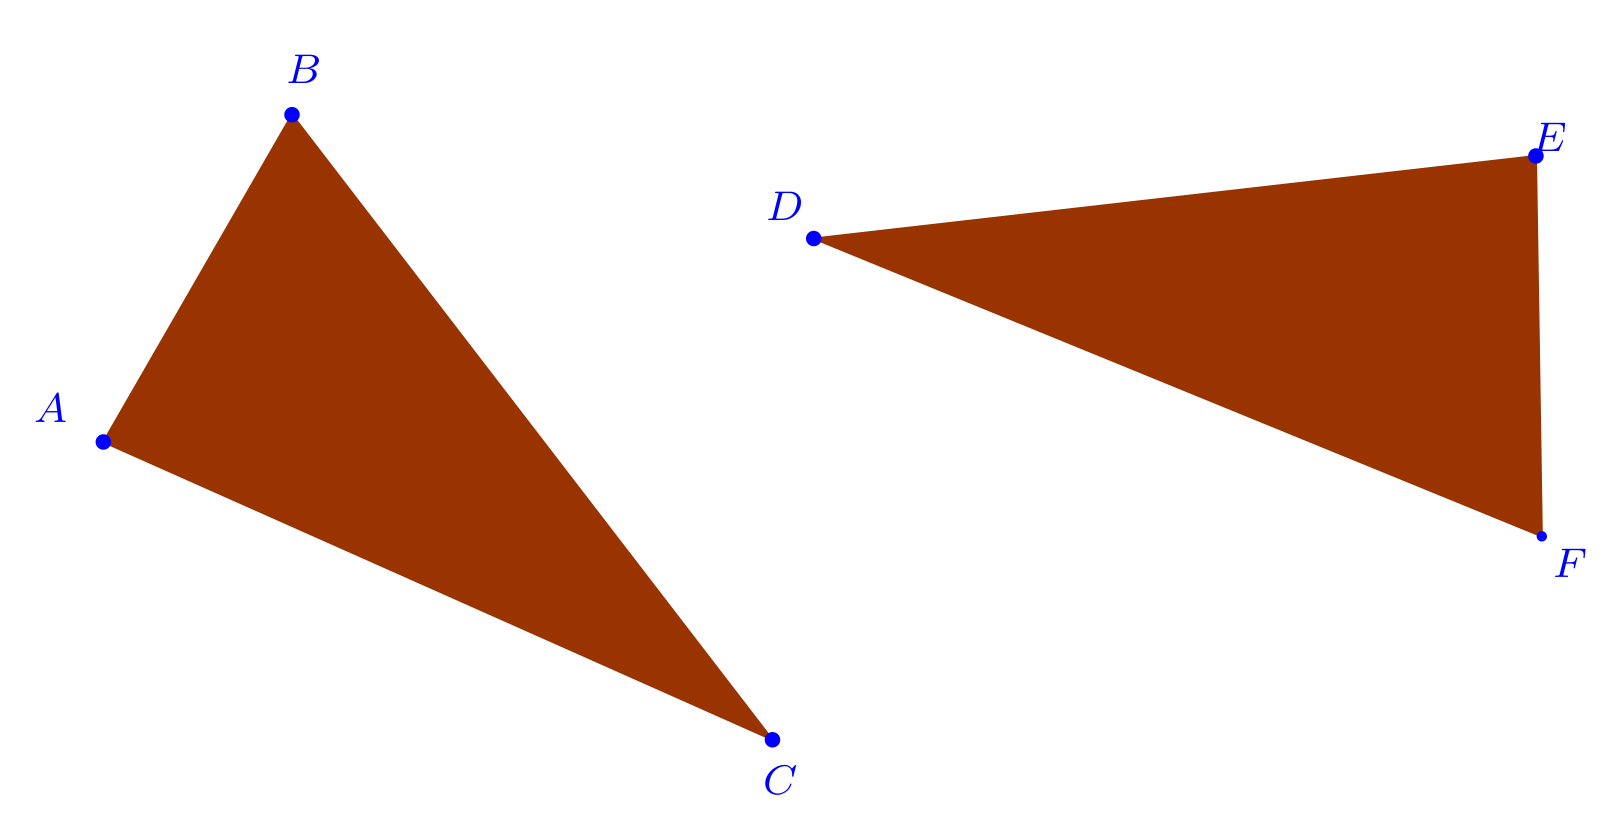
\includegraphics[width=0.9\linewidth]{3x2-triangles-semblables/ex1.png}
\end{figure}

\subsubsection*{Ex2}

Démontrer que les triangles sont semblables.

\begin{figure}[H]
      \centering
      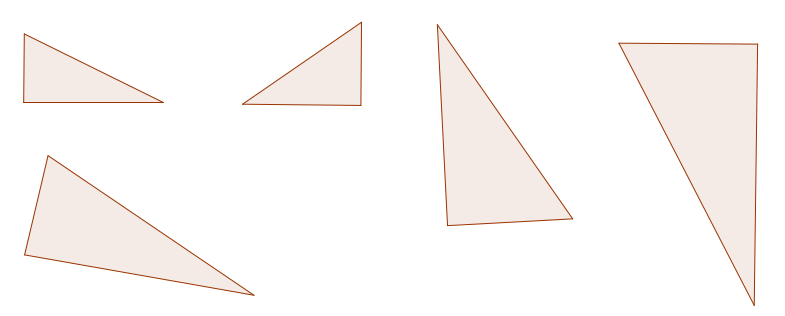
\includegraphics[width=\linewidth]{3x2-triangles-semblables/ex2.png}
\end{figure}

\end{multicols}
\begin{multicols}{2}
\subsubsection*{Ex3}

Les triangles sont semblables. Calculer les longueurs manquantes.

\begin{figure}[H]
      \centering
      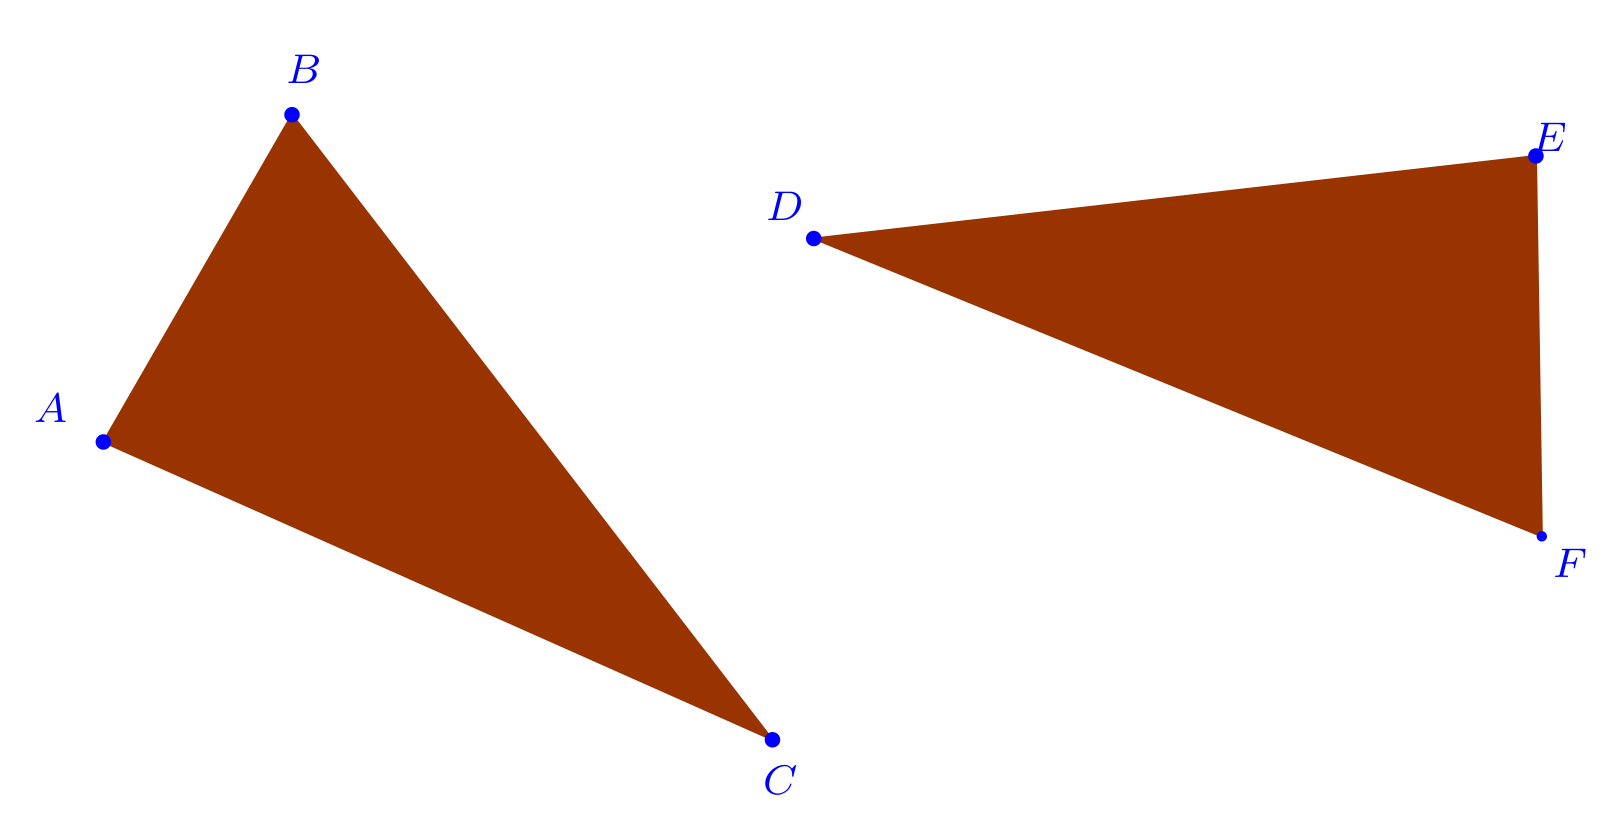
\includegraphics[width=0.9\linewidth]{3x2-triangles-semblables/ex1.png}
\end{figure}


\subsubsection*{Ex4}

Les triangles sont semblables. Calculer les longueurs manquantes.

\begin{figure}[H]
      \centering
      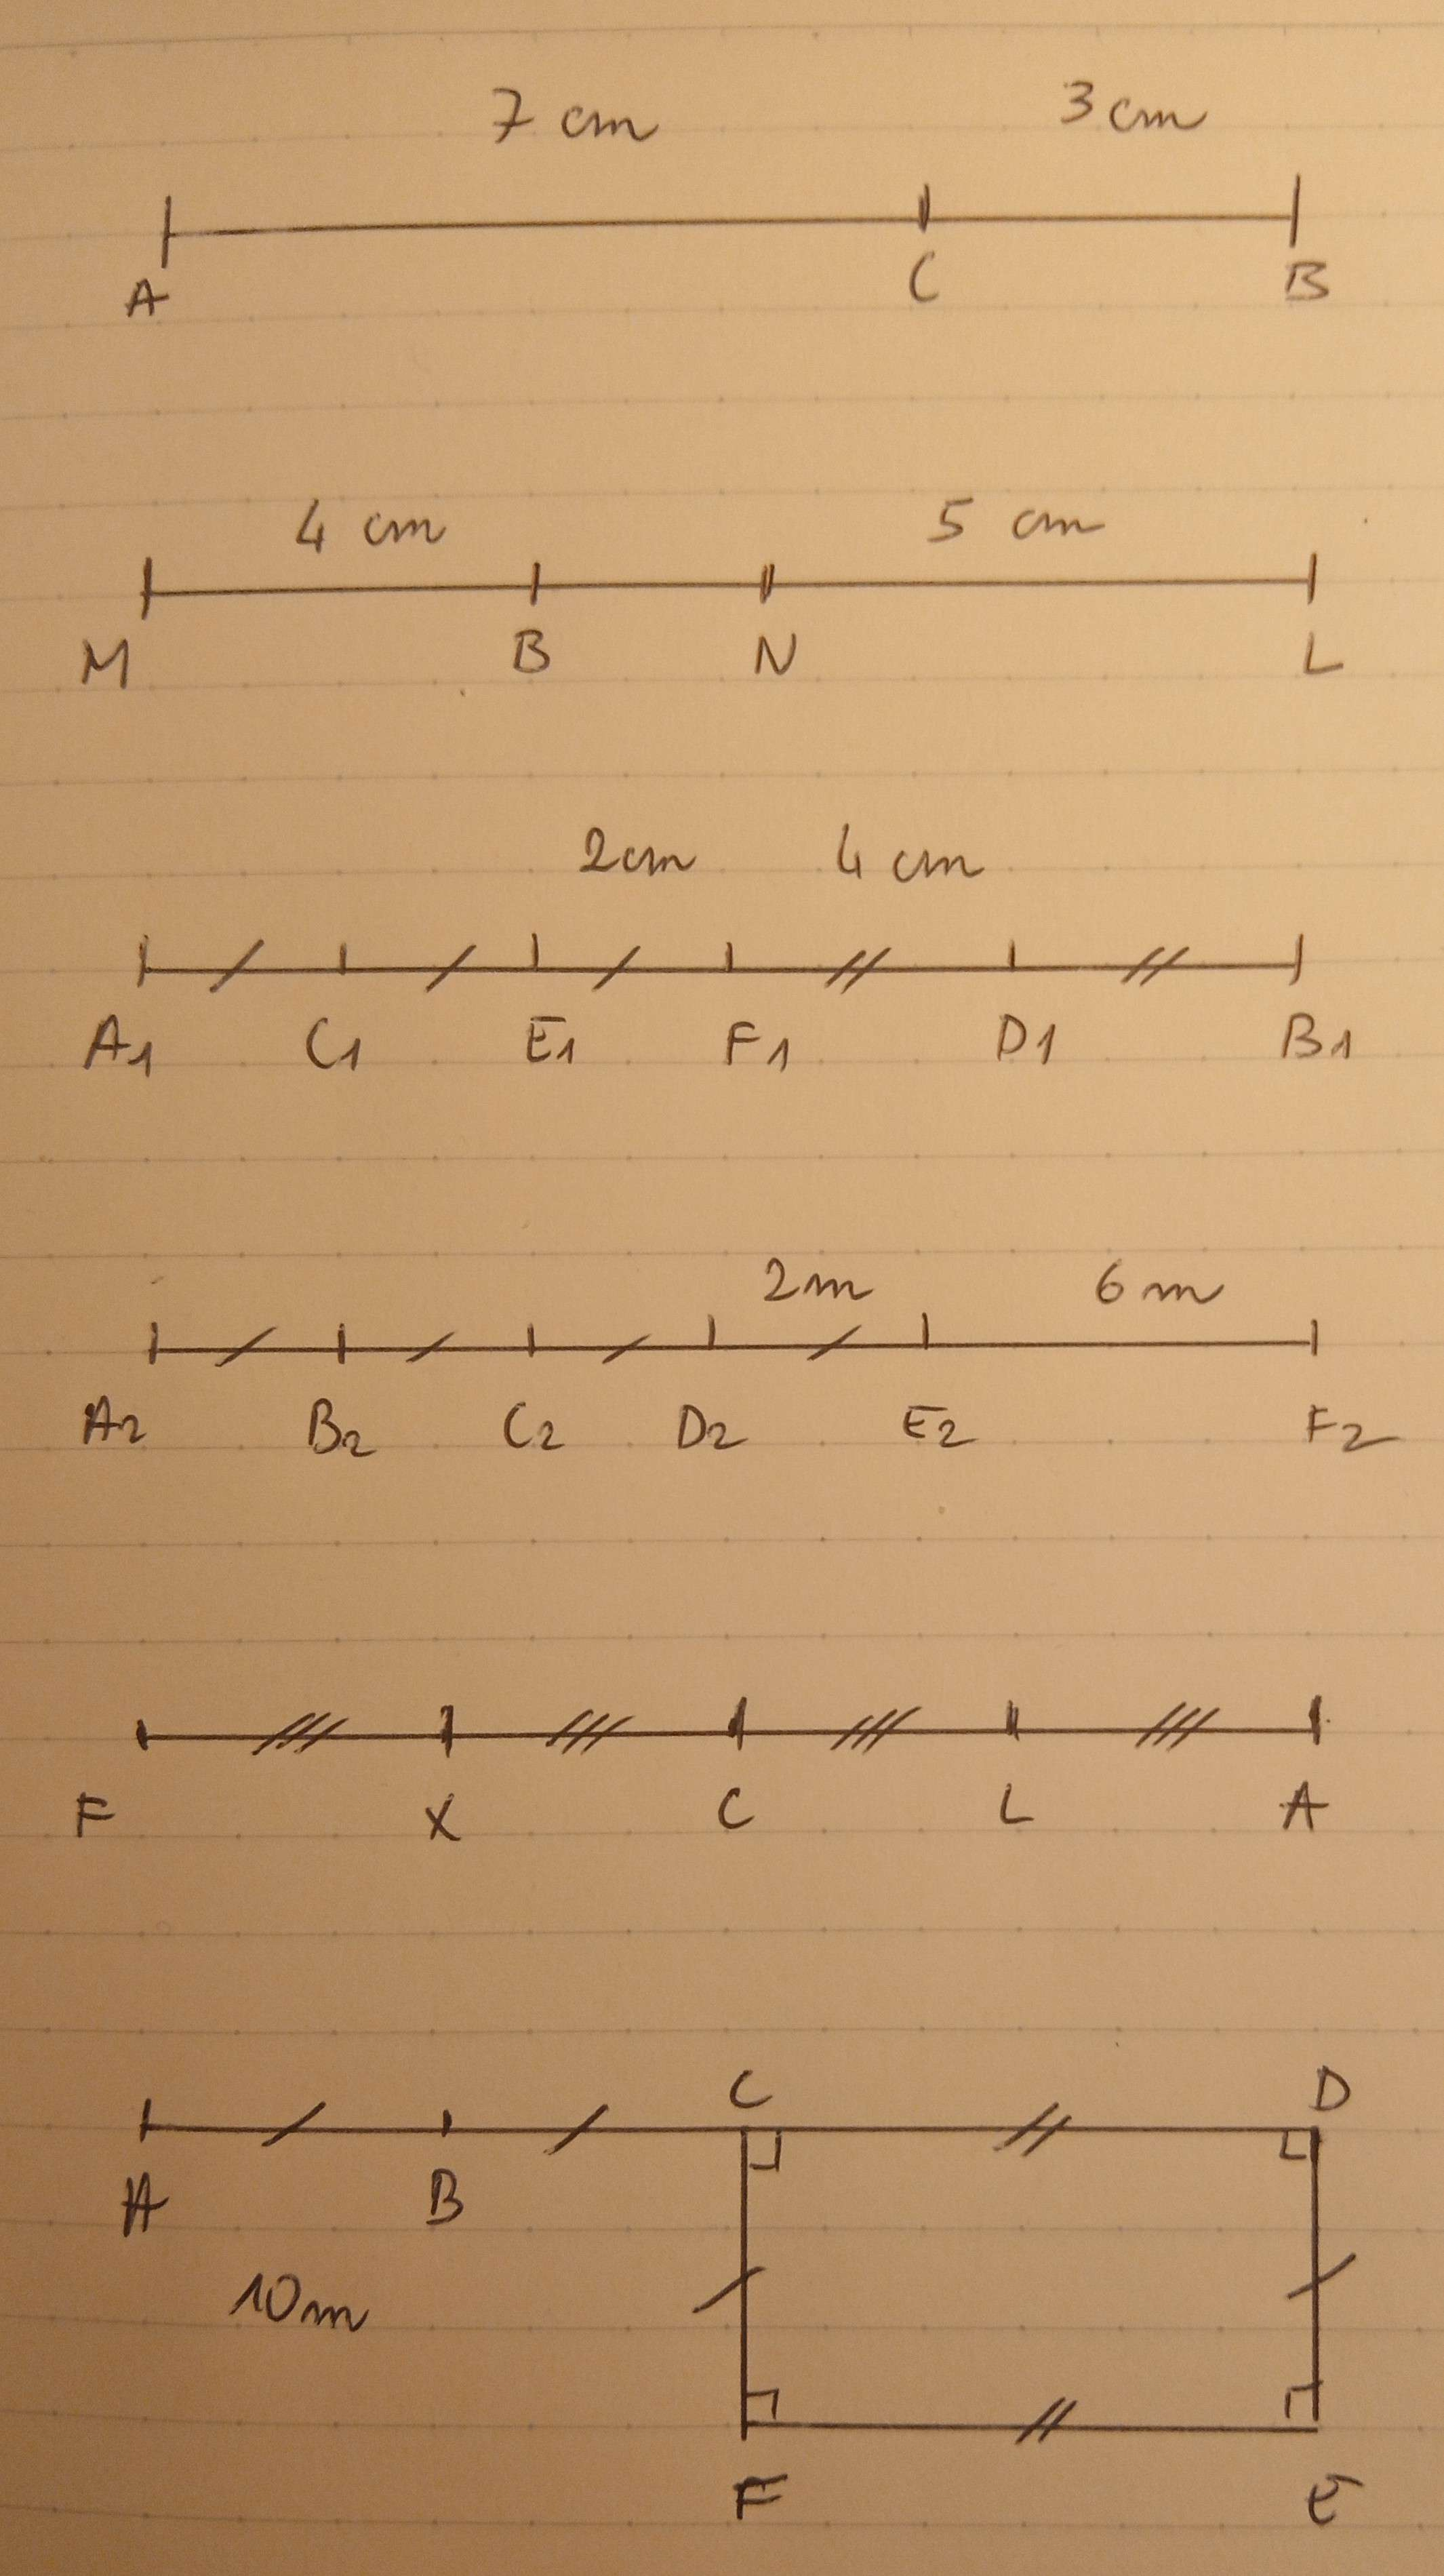
\includegraphics[width=\linewidth]{3x2-triangles-semblables/ex3.png}
\end{figure}

\end{multicols}


\end{document}
